%Version 3 October 2023
% See section 11 of the User Manual for version history
%
%%%%%%%%%%%%%%%%%%%%%%%%%%%%%%%%%%%%%%%%%%%%%%%%%%%%%%%%%%%%%%%%%%%%%%
%%                                                                 %%
%% Please do not use \input{...} to include other tex files.       %%
%% Submit your LaTeX manuscript as one .tex document.              %%
%%                                                                 %%
%% All additional figures and files should be attached             %%
%% separately and not embedded in the \TeX\ document itself.       %%
%%                                                                 %%
%%%%%%%%%%%%%%%%%%%%%%%%%%%%%%%%%%%%%%%%%%%%%%%%%%%%%%%%%%%%%%%%%%%%%

%%\documentclass[referee,sn-basic]{sn-jnl}% referee option is meant for double line spacing

%%=======================================================%%
%% to print line numbers in the margin use lineno option %%
%%=======================================================%%

%%\documentclass[lineno,sn-basic]{sn-jnl}% Basic Springer Nature Reference Style/Chemistry Reference Style

%%======================================================%%
%% to compile with pdflatex/xelatex use pdflatex option %%
%%======================================================%%

%%\documentclass[pdflatex,sn-basic]{sn-jnl}% Basic Springer Nature Reference Style/Chemistry Reference Style


%%Note: the following reference styles support Namedate and Numbered referencing. By default the style follows the most common style. To switch between the options you can add or remove “Numbered” in the optional parenthesis. 
%%The option is available for: sn-basic.bst, sn-vancouver.bst, sn-chicago.bst%  
 
%%\documentclass[sn-nature]{sn-jnl}% Style for submissions to Nature Portfolio journals
%%\documentclass[sn-basic]{sn-jnl}% Basic Springer Nature Reference Style/Chemistry Reference Style
\documentclass[pdflatex,sn-mathphys-num]{sn-jnl}% Math and Physical Sciences Numbered Reference Style 
%%\documentclass[sn-mathphys-ay]{sn-jnl}% Math and Physical Sciences Author Year Reference Style
%%\documentclass[sn-aps]{sn-jnl}% American Physical Society (APS) Reference Style
%%\documentclass[sn-vancouver,Numbered]{sn-jnl}% Vancouver Reference Style
%%\documentclass[sn-apa]{sn-jnl}% APA Reference Style 
%%\documentclass[sn-chicago]{sn-jnl}% Chicago-based Humanities Reference Style

%%%% Standard Packages
%%<additional latex packages if required can be included here>

\DeclareUnicodeCharacter{30FB}{\ensuremath{\cdot}}
\usepackage{graphicx}%
\usepackage{multirow}%
\usepackage{amsmath,amssymb,amsfonts}%
\usepackage{amsthm}%
\usepackage{mathrsfs}%
\usepackage[title]{appendix}%
\usepackage{xcolor}%
\usepackage{textcomp}%
\usepackage{manyfoot}%
\usepackage{booktabs}%
\usepackage{algorithm}%
\usepackage{algorithmicx}%
\usepackage{algpseudocode}%
\usepackage{listings}%
%%%%

%%%%%=============================================================================%%%%
%%%%  Remarks: This template is provided to aid authors with the preparation
%%%%  of original research articles intended for submission to journals published 
%%%%  by Springer Nature. The guidance has been prepared in partnership with 
%%%%  production teams to conform to Springer Nature technical requirements. 
%%%%  Editorial and presentation requirements differ among journal portfolios and 
%%%%  research disciplines. You may find sections in this template are irrelevant 
%%%%  to your work and are empowered to omit any such section if allowed by the 
%%%%  journal you intend to submit to. The submission guidelines and policies 
%%%%  of the journal take precedence. A detailed User Manual is available in the 
%%%%  template package for technical guidance.
%%%%%=============================================================================%%%%

%% as per the requirement new theorem styles can be included as shown below

\newtheorem{theorem}{Theorem}%  meant for continuous numbers
%%\newtheorem{theorem}{Theorem}[section]% meant for sectionwise numbers
%% optional argument [theorem] produces theorem numbering sequence instead of independent numbers for Proposition
\newtheorem{proposition}[theorem]{Proposition}% 
%%\newtheorem{proposition}{Proposition}% to get separate numbers for theorem and proposition etc.


\newtheorem{example}{Example}%
\newtheorem{remark}{Remark}%


\newtheorem{definition}{Definition}%

\raggedbottom
%%\unnumbered% uncomment this for unnumbered level heads

\begin{document}

\title[Article Title]{Multimodal Fusion: Advancing Medical Visual Question Answering}

%%=============================================================%%
%% GivenName	-> \fnm{Joergen W.}
%% Particle	-> \spfx{van der} -> surname prefix
%% FamilyName	-> \sur{Ploeg}
%% Suffix	-> \sfx{IV}
%% \author*[1,2]{\fnm{Joergen W.} \spfx{van der} \sur{Ploeg} 
%%  \sfx{IV}}\email{iauthor@gmail.com}
%%=============================================================%%

\author[1]{\fnm{Anjali} \sur{Mudgal}}\email{amudgal26@gwu.edu}
\equalcont{These authors contributed equally to this work.}

\author*[1]{\fnm{Udbhav} \sur{Kush}}\email{ukush4@gwu.edu}
\equalcont{These authors contributed equally to this work.}

\author[1]{\fnm{Aditya} \sur{Kumar}}\email{aditya\_kumar@gwu.edu}
\equalcont{These authors contributed equally to this work.}

\author[1]{\fnm{Amir} \sur{Jafari}}\email{ajafari@gwu.edu}

\affil[1]{\orgdiv{Department of Data Science}, \orgname{The George Washington University}, \state{Washington DC}, \country{USA}}


%%==================================%%
%% Sample for unstructured abstract %%
%%==================================%%

\abstract{This paper explores the application of Visual Question Answering (VQA) technology, which combines computer vision and natural language processing, in the medical domain, specifically for analyzing radiology scans. VQA can facilitate medical decision-making and improve patient outcomes by accurately interpreting medical imaging, which requires specialized expertise and time. The paper proposes developing an advanced VQA system for medical datasets using the Bootstrapping Language-Image Pre-training for Unified Vision-Language Understanding and Generation (BLIP) architecture from Salesforce, leveraging deep learning and transfer learning techniques to handle the unique challenges of medical/radiology images. The paper discusses the underlying concepts, methodologies, and results of applying the BLIP architecture and fine-tuning approaches for Visual Question Answering in the medical domain, highlighting their effectiveness in addressing the complexities of VQA tasks for radiology scans. Inspired by the BLIP architecture from Salesforce, we propose a novel multimodal fusion approach for medical visual question answering and evaluating its promising potential.}

%%================================%%
%% Sample for structured abstract %%
%%================================%%

% \abstract{\textbf{Purpose:} The abstract serves both as a general introduction to the topic and as a brief, non-technical summary of the main results and their implications. The abstract must not include subheadings (unless expressly permitted in the journal's Instructions to Authors), equations or citations. As a guide the abstract should not exceed 200 words. Most journals do not set a hard limit however authors are advised to check the author instructions for the journal they are submitting to.
% 
% \textbf{Methods:} The abstract serves both as a general introduction to the topic and as a brief, non-technical summary of the main results and their implications. The abstract must not include subheadings (unless expressly permitted in the journal's Instructions to Authors), equations or citations. As a guide the abstract should not exceed 200 words. Most journals do not set a hard limit however authors are advised to check the author instructions for the journal they are submitting to.
% 
% \textbf{Results:} The abstract serves both as a general introduction to the topic and as a brief, non-technical summary of the main results and their implications. The abstract must not include subheadings (unless expressly permitted in the journal's Instructions to Authors), equations or citations. As a guide the abstract should not exceed 200 words. Most journals do not set a hard limit however authors are advised to check the author instructions for the journal they are submitting to.
% 
% \textbf{Conclusion:} The abstract serves both as a general introduction to the topic and as a brief, non-technical summary of the main results and their implications. The abstract must not include subheadings (unless expressly permitted in the journal's Instructions to Authors), equations or citations. As a guide the abstract should not exceed 200 words. Most journals do not set a hard limit however authors are advised to check the author instructions for the journal they are submitting to.}

\keywords{Medical Visual Question Answering (VQA), Medical image, Multimodal Transformer, Vision Language Model, Magnetic Resonance Imaging (MRI), Computed Tomography Scan (CT Scan)}

%%\pacs[JEL Classification]{D8, H51}

%%\pacs[MSC Classification]{35A01, 65L10, 65L12, 65L20, 65L70}

\maketitle
\section{Introduction}\label{sec1}

Recent years have seen remarkable progress in computer vision and natural language processing, enabling AI systems to tackle multimodal tasks requiring a joint understanding of visual and textual data. One such challenging task is visual question answering (VQA), where a system must accurately answer questions posed in natural language about the content of a given image. It involves understanding the content of the image and correlating it with the context of the question asked. Because we need to compare the semantics of information present in both modalities — the image and natural language question related to it — VQA entails a wide range of sub-problems in both Computer Vision (CV) and Natural Language Processing (NLP) (such as object detection and recognition, scene classification, counting, and so on). Thus, it is considered an AI-complete task \cite{sahu2022vqa}.

Inspired by the success of VQA in general domains, there is growing interest in developing VQA capabilities specifically for the medical field - an area known as medical visual question answering (Med-VQA). In Med-VQA, the system receives a medical image, typically a radiology scan, along with a question in natural language, and it must provide a relevant answer by reasoning over the visual and textual inputs. While promising initial advances has been made, as highlighted by the introduction of the ImageCLEF\cite{ImageCLEFVQA-Med2019} Med-VQA challenge in 2018, the Med-VQA field is still nascent and significant research is needed before such systems can be reliably deployed in real clinical settings.
The medical field has undergone a data revolution, with electronic health records (EHRs) providing patients unprecedented access to their own medical data and imaging records. This increased accessibility enables patients to review their medical information independently, outside of formal consultations with healthcare professionals. However, this raises the need for intuitive methods that allow patients to understand and gain insights from their complex medical data without expert oversight. While patients could consult doctors, this is often impractical due to time and financial constraints. Alternatively, they may turn to general search engines or conversational AI, but risk receiving misleading or inaccurate information. To bridge this gap, Med-VQA systems could prove invaluable by allowing patients to pose natural language questions about their medical images and receive reliable answers in an accessible format.

A significant challenge faced is the limited availability of large-scale annotated Med-VQA datasets, which can impede effective learning of patterns by models. As a potential solution, pretraining and fine-tuning strategies play a crucial role in boosting performance by providing a strong initial starting point and domain-specific feature representation. Nonetheless, medical data exhibits unique characteristics that differentiate it from general domains. We hypothesize that pretraining and fine-tuning portions of a larger architecture specifically on medical data could yield performance benefits for Med-VQA by imbuing them with domain-specific knowledge more directly applicable to this specialized task.

In this research paper, we delve into the application of VQA technology to medical scans, focusing primarily on the BLIP architecture developed by Salesforce. We make the following contributions:
\begin{enumerate}
\item We combine the ImageCLEF dataset with the VQA-RAD\cite{vqa_rad} dataset which are part of a common database known as the MedPix database. We remove redundant images and retain unique scans and associated question-answer pairs. Further, we perform simple data augmentation that is appropriate for such scans to create a larger database for Med-VQA. Details of these datasets and augmentations are provided in later sections.
\item We utilize BLIP architecture from Salesforce for Med-VQA and perform answer generation as opposed to classification for Med-VQA. We further dissect this architecture, fine-tuning specific components to enhance performance.
\item Lastly, we propose a new transformer-based architecture, taking inspiration from BLIP, tailored specifically for medical image analysis. To do this, we created our own medical tokenizer based on the training data.
\end{enumerate}
The rest of the paper is organized as follows: in section 2 relevant background is briefly reviewed; in section 3 details about the methodology are provided; in section 4 experimental results are presented. Finally, section 5 concludes this paper.

\section{Background}\label{sec2}

\subsection{Literature review of Visual Question Answering}\label{subsec2.1}

Visual Question Answering (VQA) is a task that combines computer vision and natural language processing (NLP). In this task, a computer is shown an image and a question about that image in natural language. The goal is for the computer to correctly answer the question based on the information in the image \cite{agrawal2016vqa}\cite{DBLP:journals/corr/ZhangGSBP15}\cite{zhu2016visual7w}\cite{yu2015visual}.
There are different variations of VQA:
\begin{enumerate}
\item Binary (yes/no) VQA: The computer must answer the question with either "yes" or "no" \cite{agrawal2016vqa}\cite{DBLP:journals/corr/ZhangGSBP15}.
\item Multiple-choice VQA: The computer is given a set of answers and must choose the correct one \cite{agrawal2016vqa}\cite{zhu2016visual7w}.
\item Fill-in-the-blank VQA: The computer is given a statement about the image with one or more blanks, and it must fill in the missing words to complete the statement correctly \cite{yu2015visual}.
\end{enumerate}

Joint embedding approaches, inspired by advancements in deep neural networks for both computer vision and natural language processing (CNNs and RNNs), aim to learn embeddings of images and sentences in a shared feature space. This enables feeding them into a classifier together for predicting answers (\cite{gao2015talking}\cite{andreas-etal-2016-learning}). Attention mechanisms, building upon this concept (\cite{andreas-etal-2016-learning}\cite{chen2016abccnn}\cite{zhu2016visual7w}), further refine the process by concentrating on specific parts of the input, drawing inspiration from successful implementations of image captioning (\cite{xu2016show}).
Multimodal models can be of various forms to capture information from the text and image modalities, along with some cross-modal interaction as well. In fusion models, the information from the text and image encoders are fused into a combined representation to perform the downstream task.

A typical fusion model for a VQA system involves the following steps:
\begin{enumerate}
\item Featurization of image and question: We need to extract features from the image and obtain the embeddings of the question after tokenization. The question can be featurized using simple embeddings (like GLoVe), Seq2Seq models (like LSTMs), or transformers. Similarly, the image features can be extracted using simple CNNs (convolutional neural networks), early layers of object detection or image classification models, or image transformers.
\item Feature fusion: Since VQA involves a comparison of the semantic information present in the image and the question, there is a need to jointly represent the features from both modalities. This is usually accomplished through a fusion layer that allows cross-modal interaction between image and text features to generate a fused multimodal representation.
\item Answer generation: Depending on the modeling of the VQA task, the correct answers could either be generated purely using natural language generation (for longish or descriptive answers) or using a simple classifier model (for one-word/phrase answers present in a fixed answer space).
\end{enumerate}


The simple classifier approach for answer generation is inherently limited by its fixed answer space, restricting flexibility. Therefore, we explore decoder models that can generate free-form natural language answers, more suitable for complex medical reasoning. Additionally, we investigate late fusion techniques, as we believe separate bulky encoders can better capture rich representations from medical images and text before fusing them, compared to fusing from simple encoders. We hypothesize this late, powerful multimodal fusion can enhance Med-VQA performance. 

\subsection{BLIP Architecture}\label{subsec2.2}
BLIP (Bootstrapping Language-Image Pre-training) \cite{li2022blip} is a pre-training framework for unified vision-language understanding and generation, which achieves state-of-the-art results on a wide range of vision-language tasks.


Vision-language pre-training has emerged as an effective approach, where deep neural network models are pre-trained on large scale image-text datasets to improve performance on downstream vision-language tasks, such as image-text retrieval, image captioning, and visual question answering \cite{li2022blipblog}. BLIP introduces a novel architecture called Multimodal mixture of Encoder-Decoder (MED) for effective vision-language pre-training.

To pre-train a unified vision-language model capable of both understanding and generation, BLIP introduces a multimodal mixture of encoder-decoder, a multi-task model that operates in three functionalities:
\begin{enumerate}
\item Unimodal encoders, which separately encode image and text. The model uses Vision Transformer ViT \cite{dosovitskiy2021image} which divides the input image into patches and encodes them as a sequence of embedding with addition to [CLS] token to represent the globe image feature. The text encoder is the same as BERT i.e., Mask Language Model \cite{devlin2019bert} with a [CLS] token to append the beginning of the text input to summarize the sentence.
\item Image-grounded text encoder, which injects visual information by inserting a cross-attention layer between the self-attention layer and the feed forward network for each transformer block of the text encoder. A task-specific [Encode] token is appended to the text, and the output embedding of [Encode] is used as the multimodal representation of the image-text pair \cite{li2022blipblog}.
\item Image-grounded text decoder, which replaces the bi-directional self-attention layers in the text encoder with causal self-attention layers. A special [Decode] token is used to signal the beginning of a sequence \cite{li2022blipblog}.
\end{enumerate}

BLIP jointly optimizes three objectives during pre-training, with two understanding-based objectives (ITC, ITM) and one generation-based objective (LM):

\begin{enumerate}
\item Image-Text Contrastive Loss (ITC) activates the unimodal encoder. It aims to align the feature space of the visual transformer and the text transformer by encouraging positive image-text pairs to have similar representations in contrast to the negative pairs \cite{li2022blipblog}.
\item Image-Text Matching Loss (ITM) activates the image-grounded text encoder. ITM is a binary classification task, where the model is asked to predict whether an image-text pair is positive (matched) or negative (unmatched) given their multimodal feature \cite{li2022blipblog}.
\item Language Modeling Loss (LM) activates the image-grounded text decoder, which aims to generate textual descriptions conditioned on the images \cite{li2022blipblog}.
\end{enumerate}

To perform efficient pre-training while leveraging multi-task learning as explained above:

\begin{enumerate}
\item The text encoder and text decoder share all parameters except for the self-attention layers. The reason is that the differences between the encoding and decoding tasks are best captured by the self-attention layers.
\item The encoder employs bi-directional self-attention to build representations for the current input tokens,
\item while the decoder employs causal self-attention to predict the next tokens.
\end{enumerate}

For the task of Visual Question Answering (VQA), BLIP formulates it as an answer generation problem. During fine-tuning, the pre-trained model encodes an image-question pair into multimodal embeddings using the image-grounded text encoder, which are then passed to the answer decoder to generate the answer. The VQA model is fine-tuned using the language modeling (LM) loss with ground-truth answers as targets \cite{li2022blip}.

BLIP achieves state-of-the-art performance on the VQA task, outperforming models like ALBEF \cite{li2021align} and SimVLM \cite{wang2022simvlm}, even when using significantly less training data. The success of BLIP is attributed to its effective MED architecture and joint pre-training approach, which enables seamless transfer learning to downstream tasks like VQA.

The BLIP model architecture consists of layers that process both visual and textual inputs in a unified manner.

\begin{itemize}
    \item Visual Processing: Pass the visual features extracted from the images through a visual encoder network, which captures the visual information.
    \item Textual Processing: Process the encoded textual data through a textual encoder network, which understands the semantic meaning of the text.
    \item Fusion: Combine the visual and textual representations using fusion mechanisms such as attention mechanisms or multi-modal fusion layers. This step aims to create a joint representation that captures the correlation between the visual and textual modalities.
\end{itemize}

\section{Methodology}\label{sec3}
\subsection{Dataset}\label{subsec3.1}

Our research capitalizes on a unified dataset derived from two closely related sources: ImageCLEF 2019 and VQA-RAD. Both ImageCLEF 2019 and VQA-RAD datasets serve as pillars of our investigation, offering a curated compilation of radiology images coupled with corresponding question-answer pairs. Despite their separate identities, these datasets share fundamental characteristics, focusing on radiological examinations and encompassing a spectrum of anatomical structures and medical scenarios. These datasets are characterized by their emphasis on four primary question types: Modality, Plane, Organ system, and Abnormality. Through this categorization, it offers a structured approach to querying medical images, enhancing interpretability, and facilitating targeted investigations.

Recognizing the intrinsic similarities between ImageCLEF2019 and VQA-RAD, we adopted a strategy of dataset consolidation to streamline our analysis. By merging the pertinent components of both datasets, we constructed a cohesive corpus tailored to our research objectives. This consolidation process facilitated a more coherent and comprehensive examination of medical image understanding and interpretation. Also, to ensure data integrity, we removed redundant images and question answer pairs from our combined dataset. 
After consolidating the datasets, our combined corpus comprises 14,590 question-answer pairs in the training set, 2,000 pairs in the validation set, and 500 pairs in the test set.

A sample from the ImageCLEF 2019 dataset:
\begin{figure}[h]
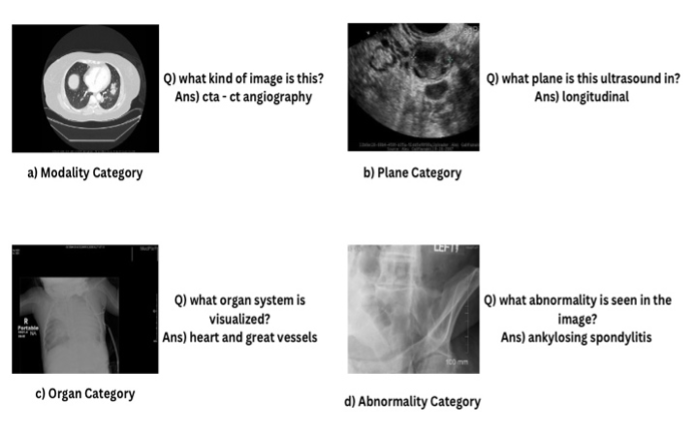
\includegraphics[width=0.6\textwidth]{figs/representative_imageclef.png}
\caption{Representative Image Samples from ImageCLEF}
\centering
\end{figure}

\subsubsection{Augmentation}\label{subsubsec3.1.1}
Due to the limited number of original medical scans available in our dataset, we employed image augmentation techniques to expand our dataset and enhance the quality of image embeddings. Image augmentation involves applying transformations to the original images to create new variations while preserving their semantic content.

For our augmentation process, we applied transformations such as blur, brightness adjustment, and noise addition to each original image. These transformations help to introduce variability in the dataset, which can improve the robustness and generalization ability of our machine learning models trained on the augmented data.

\begin{figure}[h]
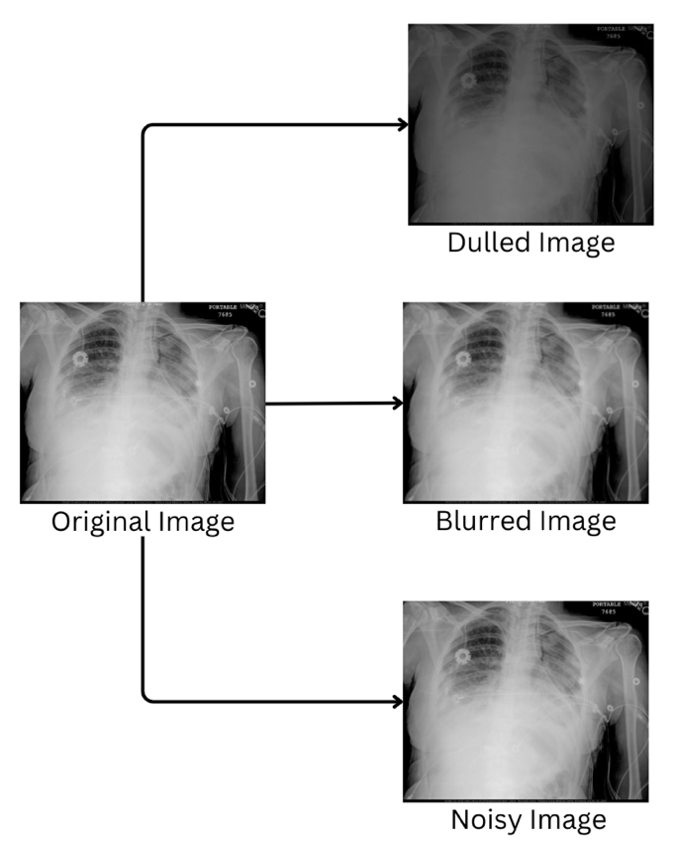
\includegraphics[width=0.6\textwidth]{figs/augmentation.png}
\caption{Augmentation of the Images from the Train Dataset Sample}
\centering
\end{figure}

To expand our training set, we applied augmentation techniques to each of the 3,200 original images, resulting in the creation of three additional images per original image through blur, 
brightness adjustment, and noise addition. This process yielded an additional 9,600 images, effectively tripling the size of our training dataset. The final size of our training set is 24,190 question-answer pairs, validation set is 2,000 question-answer pairs and test set are 500 question-answer pairs.


\subsection{BLIP Fine-Tuning}\label{subsec3.2}
To start the analysis, we used the BLIP pre-trained model for question-answering from HuggingFace to run an evaluation loop or inference on the test data created while preprocessing the ImageCLEF and VQA-RAD datasets. The corresponding BLIP processor is utilized from HuggingFace on the image-question and answer pair. The BLIP processor wraps a BERT tokenizer and BLIP image processor into a single processor. The image processor performs preprocessing on our medical images according to the BLIP pre-training transformations and BERT tokenizer converts the questions and answers to corresponding token ids according to the vocabulary of this tokenizer. A batch size of 12 is used to run this inference. With this we benchmark the performance of BLIP pre-trained model, that has been trained on COCO dataset and Visual Genome datasets \cite{krishna2016visual}, on medical radiology scans. This serves as the baseline performance of BLIP pre-trained Visual Question Answering architecture for medical domain. The architectural flow of image-question in BLIP for VQA has been discussed in section 2.2. The performance metrics used for the Visual Question Answering tasks are BLEU score \cite{10.3115/1073083.1073135} and ROUGE score \cite{lin-2004-rouge} which have been noted down in the results section below. 

After this, we fine-tuned BLIP for question-answering on our medical dataset. All the model weights and biases are unfrozen to achieve this. We use the 24,190 question-answer pairs in the training set, and 2,000 pairs in the validation set to perform this fine-tuning as discussed in section 3.1. This fine-tuning was performed for a batch size of 12, and for 15 epochs. However, the model parameters seem to converge within the first 5 epochs when saved on the validation cross-entropy loss which is the Language Model loss discussed in section 2.2. The image-question and answer follow the same processor steps that have been described above. AdamW \cite{loshchilov2019decoupled} is used as the optimizer with a learning rate of 4e-5 along with an exponential learning rate scheduler with a gamma value of 0.9. After the best model was saved, a similar inference or evaluation loop as above is run on the test data to retrieve the benchmark metrics for this fine-tuned BLIP model. The results and discussion are noted down below.

\subsection{BLIP Vision Encoder – Incorporating Medical Domain Knowledge}\label{subsec3.3}
\begin{figure}[h]
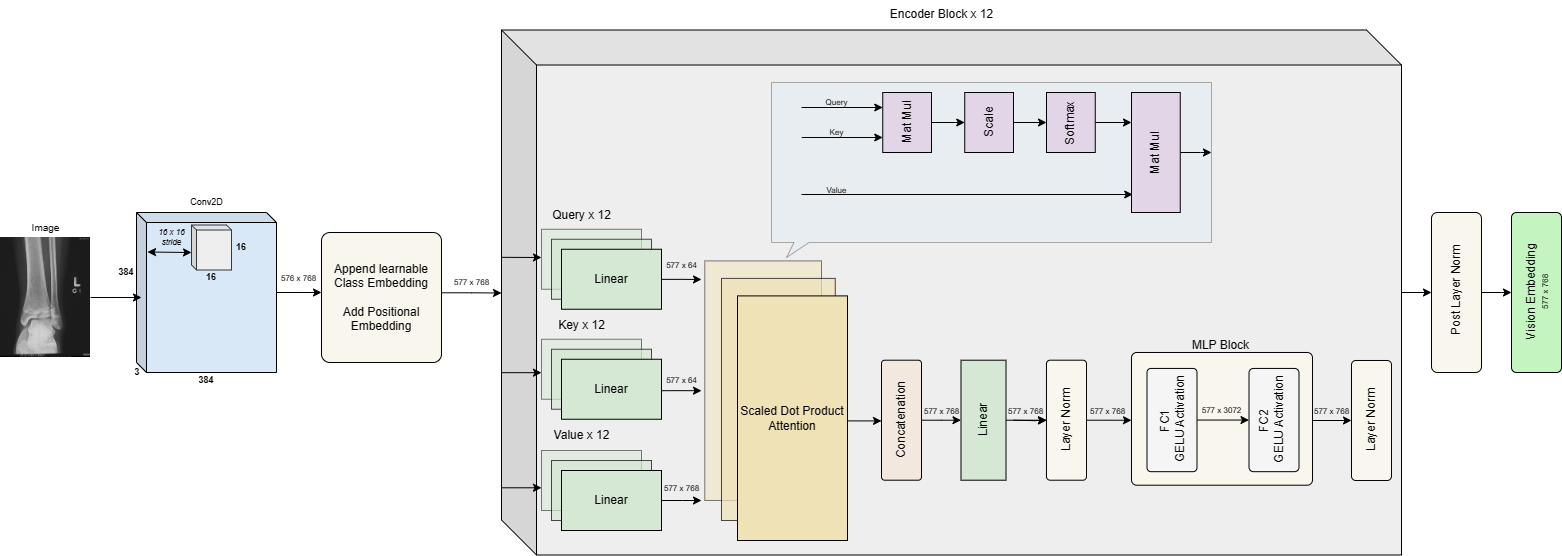
\includegraphics[width=1.0\textwidth]{figs/BLIPVision_final.drawio.png}
\caption{BLIP Vision Encoder}
\centering
\end{figure}
We observed that the process of fine-tuning the entire BLIP architecture for Visual Question Answering in medical domain was a time-consuming process where each epoch took 1 hour to run on NVIDIA A10G Tensor Core GPUs. We attempted to dissect this architecture to see whether we can perform enhancements. We first dissected the vision model and observed the different components – a patch embedding convolution layer to divide images in patches and retain patch positional encoding and the transformer encoder to create image embeddings. We decided to customize the pre-trained BLIP vision model to our specific medical task and assess its impact. The size of the convolution layer was - Conv2d(3, 768, kernel size=(16, 16), stride=(16, 16)). We created a custom autoencoder architecture starting with the same dimension as this convolution patch embedding layer. A detailed representation of the custom autoencoder architecture is given in figure 8. The purpose of this autoencoder architecture is to learn a hidden representation of all the medical radiology images by minimizing the error of reconstruction. We hypothesized that after training the custom autoencoder, the first layer of this custom architecture, which is the same size as the convolution patch embedding layer of the vision model, will learn better weights and biases that are customized to medical images. We train our custom autoencoder architecture with complete medical images, for a batch size of 64 and 10 epochs. The optimizer and scheduler are utilized as described above. We use the mean square error loss between the reconstructed and original images passed as both the input and as target. 
The learned weights are retrieved from the first layer of the custom autoencoder and are plugged into the BLIP vision model. To assess the impact of performing this specialized fine-tuning on a component of the vision model, we run an inference or evaluation loop using BLIP model for question-answering initialized with the new convolution patch embedding weights. The results are discussed in the section below. 
As the next step, we fine-tune the entire BLIP model for question-answering again using the same specifications that are discussed above, with the new addition of convolution patch embedding layer in the vision model initialized with learned weights from the custom autoencoder. This is our hypothesized contribution to improve results of the fine-tuned BLIP model for question-answering on a relatively small medical dataset. We propose fine-tuning the patch embedding layer of vision model on medical images to learn customized weights. We then apply this learned weight to the base BLIP architecture for question-answering, freezing the parameters for convolution patch embedding layer of the vision model and finally fine-tuning the remaining BLIP architecture with the medical dataset. This fine-tuning has been performed for a batch size of 12 for 10 epochs. 

\begin{figure}[h]
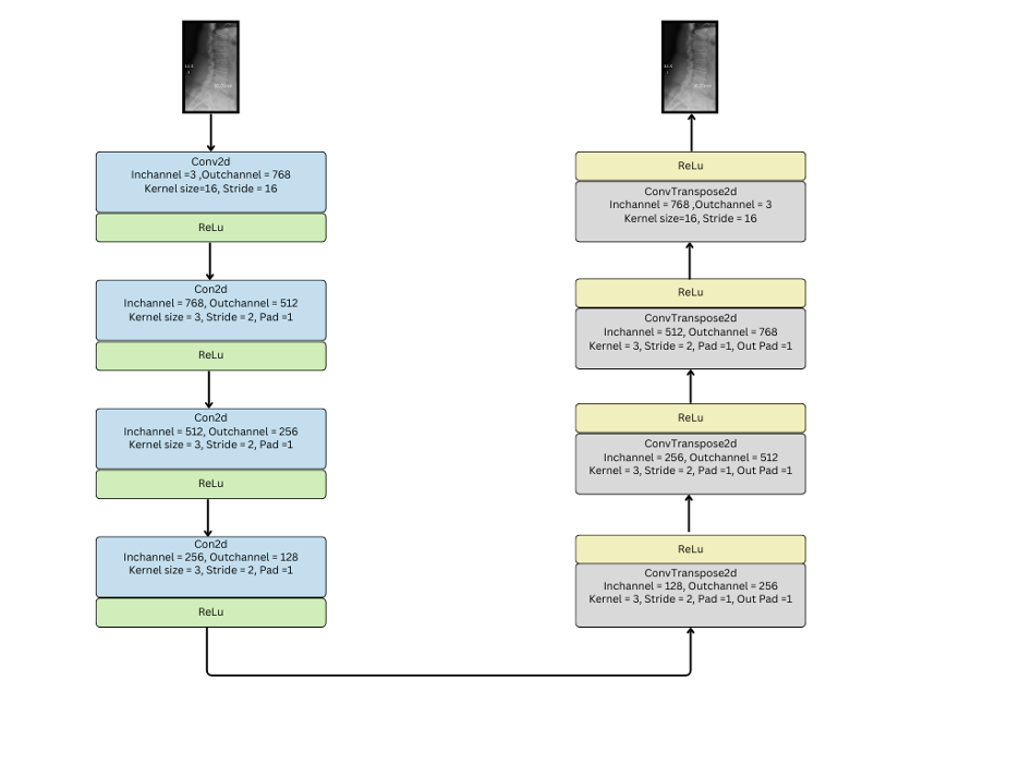
\includegraphics[width=0.9\textwidth]{figs/autoencoder.png}
\caption{Autoencoder Model to Finetune the Vision Model of BLIP VQA}
\centering
\end{figure}

\subsection{Modified BLIP for Med-VQA- Proposed Architecture}\label{subsec3.4}
Inspired by the BLIP architecture, which fuses text and vision embeddings using cross-attention, we propose a modified approach for Visual Question Answering in the medical domain. Our architecture leverages the pre-trained BLIP vision encoder to generate image embeddings and a custom transformer encoder architecture is pre-trained on our medical dataset to encode question embeddings.

\begin{figure}[h]
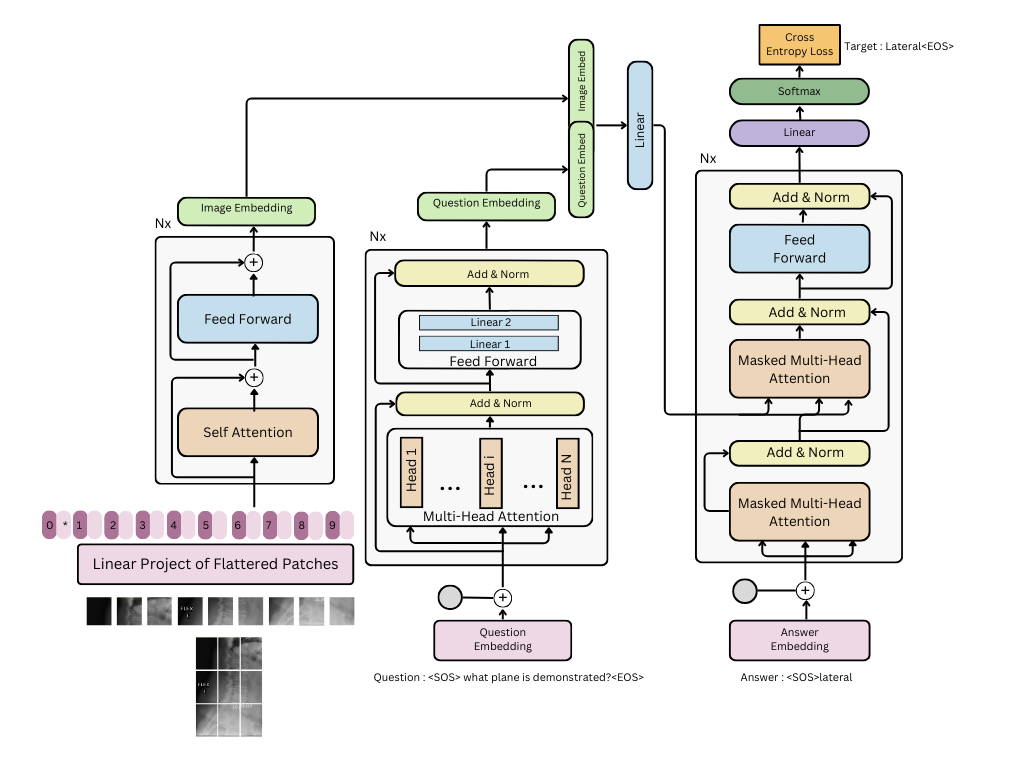
\includegraphics[width=0.9\textwidth]{figs/proposed_architecture.png}
\caption{Proposed Architecture}
\centering
\end{figure}

These embeddings are concatenated and down-sampled using a linear layer, forming a rich fused representation. The resulting embedding serves as input to the decoder, enabling the generation of accurate answers based on the combined visual and textual information. We evaluate our approach and discuss the results, highlighting the potential of this fusion technique for enhancing Visual Question Answering performance in the medical domain.

\subsubsection{Image Embedding}\label{subsubsec3.4.1}

The BLIP (Bootstrapping Language-Image Pre-training) vision model processes images through a series of steps. First, the BLIP vision processor is used to preprocess all the images, resizing them to a fixed size of 368 x 368 pixels. The preprocessed images are then passed through a convolutional layer with a kernel size of 16 and a stride of 16, resulting in a vision embedding of size 576. 

The size of the output is calculated using the convolutional formula:
\begin{equation}
    n_{\mathrm{out}}=\left\lfloor\frac{n_{\mathrm{in}}-K+2p}{S}\right\rfloor+1
\end{equation}
where $n_{\mathrm{out}}$ is the number of output channels, $n_{\mathrm{in}}$ is the number of input channels which is 3 in our case as we are dealing with an RGB image, K is the kernel size (16 in our case), p is the padding (0 in our case), and S is the stride (16 in our case).

To capture global information, an extra embedding is added at the start of the vision embedding, and positional embeddings are also incorporated. After adding the extra embedding and positional embeddings, the size of the embedding becomes 577. The BLIP vision model uses a dmodel (dimensionality of the model) of 768, projecting each patch in the vision embedding to this dimension. The final output of the BLIP vision model has a shape of (Batch\_size, 577, 768), representing the encoded visual features of the input images. These rich visual embeddings capture both local patch-level information and global context.

\subsubsection{Question and answer Embedding}\label{subsubsec3.4.2}

\paragraph{Tokenization}
To enhance the richness of the medical question embeddings, a custom vocabulary and tokenizer are constructed using the ImageCLEF medical dataset. This process involves combining both the questions and answers from the training data set. A Byte Pair Encoding (BPE) tokenizer is employed to create a specialized medical vocabulary through sub-word tokenization. BPE algorithmically identifies and combines frequently occurring sub-word units, enabling the effective handling of domain-specific terms and expressions prevalent in medical terminology. Additionally, special tokens such as PAD (padding), SOS (start of sentence), EOS (end of sentence), UNK (unknown), MASK (masked token), and SEP (separator) are incorporated into the vocabulary. Despite the limited size of the medical dataset, this approach facilitates a more comprehensive understanding of medical language by capturing the nuances and intricacies specific to the domain. By leveraging this custom vocabulary and tokenization technique, the model is equipped to process and represent medical questions with greater precision and contextual understanding.

\paragraph{Encoding}
The Transformer\cite{vaswani2023attention} Question Encoder plays a vital role in the proposed model for medical question answering. Its purpose is to process the input question and generate a dense vector representation that captures the semantic information of the question. To ensure compatibility with the visual embeddings, the question sequence length is fixed at 577, and the dimensionality of the model ($d_{\mathrm{model}}$) is set to 768.

The encoding process begins by adding special tokens to the question. The SOS (start of sentence) token is added to the beginning of the question, and the EOS (end of sentence) token is appended to the end. These special tokens help the model identify the boundaries of the question and provide a clear starting and ending point for the encoding process.

Once the special tokens are added, the question tokens are passed through an embedding layer called InputEmbeddings. This layer converts each token into a dense word embedding, transforming the discrete token representations into continuous vector representations. The word embeddings capture the semantic and syntactic information of the tokens, allowing the model to understand the meaning and relationships between the words in the question. To scale the embeddings as suggested in the original Transformer paper, the embeddings are multiplied by the square root of $d_{\mathrm{model}}$.

Next, positional encodings are added to the word embeddings using the PositionalEncoding module. Positional encoding is used in the Transformer architecture to inject sequence-wise information. The position encoding layer employs a combination of sinusoidal and cosine functions to create a geometric sequence of values.

For even positions in the range $[0, d_{\mathrm{model}}]$, a sinusoidal function is used: 
\begin{equation}
    PE(pos, 2i) = \sin(pos \times div\_term)
\end{equation}

For odd positions, a cosine function is used:
\begin{equation}
    PE(pos, 2i+1) = \cos(pos \times div\_term)
\end{equation}

Here, pos is the position index, i is an even integer in $[0,d_{\mathrm{model}}]$, and div\_term is calculated as:
\begin{equation}
    div\_term = exp(-i*(log(10000) / d_{\mathrm{model}}))
\end{equation}


The div\_term creates a geometric sequence that decreases exponentially as i increases, with the rate of decrease controlled by $log(10000) / d_{\mathrm{model}}$.

The alternating sine and cosine functions create unique embeddings for each position, allowing the model to distinguish between even and odd positions. These positional encoding values are added element-wise to the input embeddings, providing the Transformer with positional information to effectively learn and attend to the relative positions of tokens within the sequence.

After adding the positional encodings, the question embeddings are passed through the Transformer encoder. The Transformer encoder consists of multiple layers, each containing a multi-head self-attention mechanism and a feed-forward neural network.
\begin{itemize}
    \item The input embeddings and positional embeddings are added together and passed as query (Q), key (K), and value (V) matrices into the Multi-Head Attention block.
    \item Each head (h=8 in this case) has its own learned weight matrices: $W_{\mathrm{q}}$, $W_{\mathrm{k}}$, and $W_{\mathrm{v}}$. The Q, K, and V matrices are multiplied with their respective weight matrices to obtain Q', K', and V' for each head.
    \item The dimensionality of each head is reduced to $d_{\mathrm{k}} = d_{\mathrm{model}} / h$ (768/8 = 96 in this case), allowing each head to focus on a specific part of the embedding.
    \item For each head, the attention scores are computed using the scaled dot-product attention:
    $head(i) = Attention(QW_i^q, KW_i^k, VW_i^v)$
    \begin{equation}
    \mathrm{Attention}\left(Q,K,V\right)=\mathrm{softmax}\left(\frac{QK^T}{\sqrt{d_k}}\right)V
    \end{equation}
    \item The attention scores are scaled by dividing them by the square root of $d_{\mathrm{model}}$ to prevent the dot products from growing too large.
    \item The softmax function is applied to the scaled attention scores to obtain the attention weights, which are then multiplied with the value matrix (V) to get the weighted values for each head.
    \item The outputs from all heads are concatenated together:
    \begin{equation}
        \mathrm{Multihead}\left(Q,K,V\right)=\mathrm{Concat}(head_{\mathrm{1}},head_{\mathrm{2}},\text{...}, head_{\mathrm{h}})W^0
    \end{equation}

    \item The concatenated output is then multiplied with the $W^0$ matrix to obtain the final output of the Multi-Head Attention block. By using multiple heads, the Multi-Head Attention mechanism allows the model to attend to different aspects of the input embeddings simultaneously, capturing various relationships and dependencies within the sequence.
\end{itemize}

The output of the Transformer encoder is the final question embedding, which has a size of (Batch, 577, 768). This embedding size matches the dimensions of the visual embeddings, ensuring a consistent representation across both modalities. By aligning the question and visual embeddings in terms of sequence length and dimensionality, the model can effectively process and integrate the information from both sources in the subsequent stages.
The consistent representation achieved by the Transformer Question Encoder facilitates seamless interaction between the question and visual information. It allows the model to attend to relevant parts of the question and visual features simultaneously, enabling it to reason and generate accurate answers based on the combined context.
In summary, the Transformer Question Encoder is a critical component in the proposed model for medical question answering. It processes the input question, incorporates positional information, and generates a dense vector representation that captures the semantic information of the question. By ensuring consistency with the visual embeddings, the question encoder enables effective integration and interaction between the question and visual modalities, facilitating accurate and informed answering of medical questions.


\paragraph{Fusion}
The concatenation of the image embedding and question embedding results in a fused embedding that combines information from both modalities. We denote the image embedding as $E_{\mathrm{img}}$ and the question embedding as $E_{\mathrm{q}}$. The fused embedding $E_{\mathrm{fused}}$ can be represented as:
\begin{equation}
    E_{\mathrm{fused}}=\mathrm{Concat}\left(E_{\mathrm{img}},E_q\right)
\end{equation}

where $Concat()$ represents the concatenation operation along the last dimension.

The shape of the fused embedding is (Batch, 577, 768*2), as it combines the image and question embeddings, each of shape (Batch, 577, 768).
To ensure proper fusion and compatibility with the subsequent layers, a linear projection layer is applied to the fused embedding. This layer transforms the fused embedding into the desired shape of (Batch, 577, 768). We denote the linear projection layer as $L_{\mathrm{proj}}$. The projected fused embedding $E_{\mathrm{proj}}$ can be expressed as:
\begin{equation}
E_{\mathrm{proj}}=\mathrm{L}_{\mathrm{proj}}\left(E_{\mathrm{fused}}\right)
\end{equation}

where $L_{\mathrm{proj}}$ is a linear transformation that maps the fused embedding to the desired size.

The projected fused embedding $E_{\mathrm{proj}}$ is then passed to the decoder as the key (K) and value (V) pair for the attention mechanism. The query (Q) for the decoder is obtained from the input to the decoder after applying causal self-attention.
In the decoder, the input is the answer sequence, and an SOS (start of sentence) token is appended at the start of the answer to predict the next token. The decoder uses causal attention, also known as masked self-attention, which allows each token to attend only to the previous tokens in the sequence.
The attention mechanism in the decoder can be represented by the following equation:
\begin{equation}
    \mathrm{Attention}\left(Q,K,V\right)=\mathrm{softmax}\left(\frac{QK^T}{\sqrt{d_k}}\right)V
\end{equation}

\begin{equation}
    d_{k\ }=\frac{d_{model}}{number\ of\ heads}
\end{equation}

\begin{equation}
    numberofheads=8
\end{equation}

where Q represents the query matrix derived from the decoder input after causal self-attention, with shape as (Batch, sequence length of answer, $d_{\mathrm{model}}$), K represents the key matrix, which is the projected fused embedding $E_{\mathrm{proj}}$, with shape (Batch, 577, $d_{\mathrm{model}}$)), V represents the value matrix, which is also the projected fused embedding $E_{\mathrm{proj}}$, with size (Batch, 577, $d_{\mathrm{model}}$). The sequence length of the answer is the maximum number of tokens in the answer, 200 in our case.
The attention weights are computed by taking the dot product of the query and key matrices, scaling it by square root of $d_{\mathrm{k}}$, and applying a softmax function. The resulting attention weights are then used to compute a weighted sum of the value vectors, generating the attended output.

\paragraph{Decoder}
By using the projected fused embedding as the key and value pair, the decoder attends to the relevant information from both the image and question embeddings to generate the answer sequence. The causal attention mask ensures that the decoder can only attend to the previous tokens in the answer sequence, enabling auto-regressive generation of the answer.
To train the model, the widely adopted cross-entropy loss function is employed, which measures the dissimilarity between the predicted and actual probability distributions of the answer tokens. This loss function guides the model to minimize the discrepancy between its predictions and the ground truth answers. Furthermore, the BLEU score, a well-established metric in natural language processing, is utilized to evaluate the quality of the generated answers. BLEU assesses the similarity between the generated answers and the reference answers, considering factors such as n-gram precision and brevity penalty.

The proposed approach offers a novel method for generating rich embeddings that capture the essence of both the image and the question. By treating these embeddings separately and considering their relationship to the answer, the model can effectively leverage the information from both modalities to generate accurate and contextually relevant responses.

In conclusion, the proposed approach for Visual Question Answering in the medical domain introduces a novel fusion technique that combines image and question embeddings to generate accurate and contextually relevant answers. By leveraging the BLIP vision encoder for image embedding generation and pre-training a custom transformer encoder for question embedding encoding, the model captures rich visual and textual information. The concatenation and down sampling of these embeddings using a linear layer form a powerful fused representation that serves as input to the decoder. The decoder, equipped with causal attention, attends to the relevant information from the fused embedding to generate answer sequences. The incorporation of custom vocabulary through the BPE tokenizer further enhances the model's ability to handle domain-specific medical terminology. The evaluation using cross-entropy loss and BLEU score demonstrates the effectiveness of this approach in generating accurate answers. Overall, this innovative framework holds significant potential for improving the efficiency and performance of medical question-answering systems, ultimately benefiting healthcare professionals and patients by providing precise and reliable information.

\section{Experiments and Results}\label{sec4}

In this section, we demonstrate BLIP’s effectiveness on Visual Question Answering (VQA) on medical datasets such as X-rays, MRI scans, etc. by using a pre-trained base BLIP model and fine-tuning it in multiple ways to see its performance. The key idea here is to achieve good results for a low fine-tuning time and computer resources. Detailed experimental setups are given in the next section. 

\subsection{Experimentation set-up}\label{subsec4.1}

\subsubsection{Backbone model}\label{subsubsec4.1.1}
We use the BLIP Model as our base models. This model takes images and text as input and generates text as output. 
For display equations (with auto generated equation numbers)
one can use the equation or align environments:

\subsection{Metrics}\label{subsec4.2}
Two primary metrics are used to assess the performance of fine-tuned BLIP models on VQA on medical dataset. The Bilingual Evaluation Understudy (BLEU) score [17] and the Recall-Oriented Understudy for Gisting Evaluation (ROUGE) score [18]. 

\subsubsection{BLEU}\label{subsubsec4.2.1}
The (BLEU) score is a metric used to evaluate the quality of machine-generated text by comparing it to reference texts. In our research paper, we calculate the average BLEU score to assess the performance of our Visual Question Answering model in generating accurate and relevant answers.

The average BLEU score provides an overall assessment of the model's performance in generating accurate answers. By incorporating the BLEU score as an evaluation metric, we can quantitatively measure the effectiveness of our Visual Question Answering model in generating answers that closely match the ground truth answers.

Based on the BLEU paper [17], the sentence-level BLEU score is calculated as follows:
\begin{equation}
    \text{BLEU} = \text{BP} \times \exp\left(\sum_{n=1}^{N} w_n \times \log(p_n)\right)
\end{equation}


where:
BP is the brevity penalty, which is calculated as:
\begin{equation}
    \text{BP} = \begin{cases} 
1 & \text{if output length} \geq \text{reference length} \\
\exp(1 - \text{reference length} / \text{output length}) & \text{otherwise}
\end{cases}
\end{equation}

where,

N is the maximum n-gram order (typically 4)

$w_{\mathrm{n}}$ is the weight assigned to each n-gram precision (typically uniform weights, i.e., 1/N)

$p_{\mathrm{n}}$ is the modified n-gram precision, calculated as:
\begin{equation}
    p_n=\frac{\sum_{C\in\{Candidates\}}\sum_{n\mathrm{-gram}\in C}{{\mathrm{Count}}_{\mathrm{clip}}\left(n\mathrm{-gram}\right)}}{\sum_{C^\prime\in\{Candidates\}}\sum_{n-\mathrm{gram'\ }\in C^\prime}\mathrm{Count}\left(n\mathrm{-gram'}\right)}
\end{equation}

The sentence-level BLEU score is calculated by taking the geometric mean of the modified n-gram precisions and multiplying it by the brevity penalty factor. The brevity penalty penalizes candidate translations that are shorter than the reference translations, while the modified n-gram precision accounts for both the adequacy and fluency of the translation.

\subsubsection{ROUGE}\label{subsubsec4.2.2}
ROUGE (Recall-Oriented Understudy for Gisting Evaluation) is a set of metrics used to evaluate the quality of summaries or machine-generated text by comparing them to reference summaries or gold-standard texts. ROUGE measures the overlap of n-grams, word sequences, and word pairs between the generated summary and the reference summaries. 

ROUGE-L: It measures the longest common subsequence (LCS) between the generated summary and the reference summaries. The LCS is the longest sequence of words that appear in both the generated summary and the reference summaries, allowing for gaps
ROUGE scores range from 0 to 1, with higher scores indicating better overlap between the generated summary and the reference summaries. ROUGE is widely used in the evaluation of summarization tasks, machine translation, and other natural language generation tasks.

\subsection{Results}\label{subsec4.3}
\begin{itemize}
\item \textbf{Base Blip} - This is the pre-trained BLIP model that is fetched from Hugging Face. The pre-training details are available in previous sections. This pre-trained model is used to run an inference on our dataset to determine a benchmark performance. 

\item \textbf{Fine-tuned BLIP - end-to-end} - This is the fine-tuned BLIP model on our dataset. This fine-tuning code is run for a batch size of 12, and for 15 epochs. However, the model parameters seem to converge within the first 5 epochs when saved on the validation cross-entropy loss. We observe a significant boost up in BLEU and ROUGE scores when the base BLIP model is fine-tuned on medical dataset.

\item \textbf{Convolution Patch Embedding Fine-tuned + Base BLIP} - This is our first contribution in dissecting the BLIP model. As discussed previously, we have taken the first convolution patch embedding layer from the BLIP vision encoder and recreated a custom autoencoder architecture based on the dimensions of the patch embedding layer. We have fine-tuned this custom architecture on our complete medical image dataset, to achieve a better representation of this layer customized to medical application. The first layer of this fine-tuned layer matches the dimensions of the convolution patch embedding layer. The trained weights for this layer are retrieved from the custom autoencoder and the weights are plugged into the base BLIP model. This training has been performed for a batch size of 64 and 10 epochs. The training time is significantly faster. To assess the impact of performing this specialized fine-tuning, we run an inference of the base BLIP model initialized with these convolution patch embedding layer weights. We see a boost in the benchmark BLEU and ROUGE score highlighting the effectiveness of fine-tuning only a section of the BLIP architecture.

\item \textbf{Convolution Patch Embedding Fine-tuned + Fine-tuned BLIP model} - This model version is an extension to the previous version. This is our hypothesized contribution to improve results of the fine-tuned BLIP model on a relatively small medical dataset. We have proposed fine-tuning the patch embedding layer of the vision encoder on medical images to get a good medical image representation, applying this learned weight representation to the base BLIP architecture, freezing the parameters for this specific layer and finally fine-tuning the remaining BLIP architecture with the medical dataset. We see a boost in our scores when we apply this form of training as opposed to just fine-tuning. 

\item \textbf{Proposed Architecture} - After experimenting with fine-tuning specific components, we explored a different approach for combining the vision embeddings with a question-answer transformer. Instead of using the standard methods, we utilized a technique to integrate the visual and question encodings, aiming to generate more accurate and contextually relevant answers. By leveraging our custom tokenization strategy, specifically designed for the question-answer text in the medical dataset, we observed a significant improvement in the model's performance. This combination of vision and question embeddings, coupled with our domain-specific tokenization, resulted in a substantial increase in the BLEU and ROUGE scores, reaching 0.41 and 0.44 respectively. These results highlight the effectiveness of our approach in enhancing the model's ability to generate precise and coherent answers in the medical domain, demonstrating the potential of this method for improving visual question-answering systems in specialized domains.
\end{itemize}

\begin{table}[h]
\centering
\label{tab:scores}
\begin{tabular}{|c|p{5cm}|c|c|}
\hline
\textbf{S no.} & \textbf{Model Version} & \textbf{BLEU score} & \textbf{ROUGE score} \\ \hline
1. & Base BLIP & 0.12 & 0.15 \\ \hline
2. & Fine-tuned BLIP - end-to-end & 0.37 & 0.40 \\ \hline
3. & Convolution Patch Embedding Fine-tuned + Base BLIP & 0.13 & 0.17 \\ \hline
4. & Convolution Patch Embedding Fine-tuned + Fine-tuned BLIP model & 0.38 & 0.42 \\ \hline
5. & Proposed Architecture & 0.41 & 0.44 \\ \hline
\end{tabular}
\caption{Results}
\end{table}

\section{Conclusion}\label{sec5}
This research paper explored the application of Visual Question Answering (VQA) technology in the medical domain, focusing on radiology scans. By leveraging and enhancing the BLIP architecture and proposing a multimodal transformer-based architecture, we demonstrated significant improvements in generating accurate answers to questions about medical images.
However, the study has limitations, primarily the lack of large-scale annotated medical datasets. To address this, we employed data augmentation techniques and developed a custom medical tokenizer. Despite these efforts, further research, validation, and collaboration with medical experts are necessary to curate larger datasets and assess the models' performance in clinical settings.
In conclusion, this paper showcases the potential of VQA technology in revolutionizing medical radiology analysis. With continued advancements in dataset curation, architectural innovations, and extensive clinical validation, VQA systems hold great promise in empowering healthcare professionals and enhancing patient care. Future research should focus on addressing the limitations and conducting thorough clinical evaluations to facilitate the successful integration of VQA technology in real-world medical settings.





\bibliography{sn-bibliography}% common bib file
%% if required, the content of .bbl file can be included here once bbl is generated
%%\input sn-article.bbl


\end{document}
